\documentclass[spanish, 10pt,a4paper]{article}
\usepackage[spanish]{babel}
\usepackage[utf8]{inputenc}
\usepackage{textcomp}
\usepackage{hyperref}
\usepackage[pdftex]{graphicx}
\usepackage{epsfig}
\usepackage{amsmath}
\usepackage{hyperref}
\usepackage{amssymb}
\usepackage{color}
\usepackage{graphics}
\usepackage{amsthm}
\usepackage{caratula}
\usepackage{fancyhdr,lastpage}
\usepackage[paper=a4paper, left=1.4cm, right=1.4cm, bottom=1.4cm, top=1.4cm]{geometry}
\usepackage[table]{xcolor} % color en las matrices
\usepackage[font=small,labelfont=bf]{caption} % caption de las figuras en letra mas chica que el texto
\usepackage[ruled,vlined,linesnumbered]{algorithm2e}
\usepackage{listings}
\usepackage{float}
\usepackage{amsfonts}
\usepackage{upgreek}

\color{black}

%%%PAGE LAYOUT%%%
\topmargin = -1.2cm
\voffset = 0cm
\hoffset = 0em
\textwidth = 48em
\textheight = 164 ex
\oddsidemargin = 0.5 em
\parindent = 2 em
\parskip = 3 pt
\footskip = 7ex
\headheight = 20pt
\pagestyle{fancy}
\lhead{Teor\'ia de la Comunicaciones - 2015 C2 - Trabajo Pr\'actico 2} % cambia la parte izquierda del encabezado
\renewcommand{\sectionmark}[1]{\markboth{#1}{}} % cambia la parte derecha del encabezado
\rfoot{\thepage}
\cfoot{}

%spaced sections



%El siguiente paquete permite escribir la caratula facilmente
\hypersetup{
  pdftitle={ 1c2015.PLP.RTP3},
  colorlinks,
  citecolor=black,
  filecolor=black,
  linkcolor=black,
  urlcolor=black 
}

\materia{Teor\'ia de las Comunicaciones}

\titulo{Trabajo Pr\'actico 2}

\subtitulo{Teor\'ia de las Comunicaciones}

\grupo{Grupo 4}

\integrante{Ignacio Niesz}{722/10}{ignacio.niesz@gmail.com}
\integrante{Leandro Vega}{698/11}{leandrogvega@gmail.com}
\integrante{Rodrigo Cisneros}{920/10}{rodricis@hotmail.com}
\integrante{Santiago Pernigotti}{870/11}{s.a.pernigotti89@gmail.com}
 
\begin{document}
{ \oddsidemargin = 2em
	\headheight = -20pt
	\maketitle	
}
  
	\tableofcontents
	\newpage
	\section{Introducci\'on}

En este trabajo pr\'actico vamos a desarrollar una implementaci\'on propia de traceroute. Traceroute es una consola de diagn\'ostico que permite seguir el recorrido de los paquetes, conocer cada nodo (router) por el que pasa, hasta llegar un host destino. Para poder conocer la ruta que recorren los paquetes e implementarlo, vamos a necesitar tener en cuenta las siguientes herramientas:

\begin{itemize}

\item Scapy: Herramiento usada en el trabajo pr\'actico anterior. Es una utilidad escrita en Python que nos servir\'a para crear y manipular paquetes, escanear, funciones de sniffer, entre otras.

\item ICMP (Internet Control Message Protocol): Es el sub protocolo de control y notificaci\'on de errores del Protocolo de Internet (IP). Se usa para enviar mensajes de error o de control, indicando por ejemplo que un servicio determinado no está disponible, o que un router o host no puede ser localizado, o que un paquete ha llegado al destino.
\begin{figure}[h]
	\begin{center}
    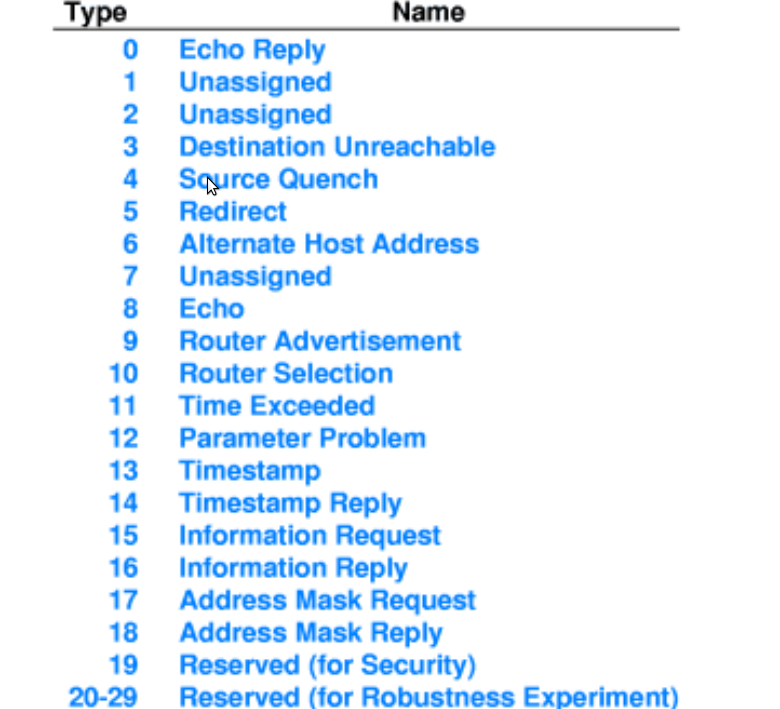
\includegraphics[width=0.5\textwidth]{ICMP_lista.png}
     \label{fig:ICMPlista} 
	\end{center}    
    \caption{Lista de algunos mensajes de control permitidos.}  
    
\end{figure}
\vspace{0.25cm}

\item TTL (time to live): No es mas que el tiempo de vida del paquete. Dentro del paquete enviado se setea dicho valor (entero) para saber cuando un paquete debe ser descartado, en caso que no llegue al destino. La forma en que funciona es: cada vez que el paquete pasa por un nodo, \'este \'ultimo le resta una unidad al valor que ten\'ia cuando lo recibi\'o, y lo propaga al siguiente nodo. En caso que el valor llegue a cero, el nodo descarta dicho paquete evitando que se siga propagando hasta su destino.

\item ICMP y TTL: Si a un paquete se le vence su TTL ($TTL = 0$), y \'este no est\'a en el nodo correspondiente a su host destino, nos llega un mensaje ICMP de "Time Exceeded" ($11$). En caso contrario, si un paquete llego a su host destino, sin importar el valor de su TTL, entonces via ICMP nos llegar\'a un mensaje de ''Echo Replay" ($0$).

\item RTT (Round-Trip delay Time): Es el tiempo que tarda un paquete de datos enviado desde un emisor en volver a este mismo, habiendo pasado por el receptor de destino. Es uno de los datos que nos muestra por pantalla las implementaciones hechas actualmente de traceroute. Con este valor podremos saber cuanto tardan los paquetes en llegar a cada nodo que intervienen en el recorrido hacia el host destino.

\end{itemize}

Una vez logrado el correcto funcionamiento del traceroute, con lo cual podremos conocer toda la ruta de un paquete, debemos tomar las estadísticas pertinentes para satisfacer los pedidos en las consignas dadas en el enunciado. Estos son:

\begin{itemize}

\item RTT promedio: Es lo que tarda un enlace en contestarnos al hacerle varias corridas, tomar diferentes tiempos y promediando dicho valor. Esto nos sirve para estimar el tiempo verdadero que tarda en llegar nuestro paquete hacia ese lugar, mitigando posibles errores en instancias particulares que pudieran darnos fuera de lo normal.

\item $\Delta$RTT: Es la diferencia entre el RTT promedio de un nodo con respecto a su antecesor.

\item Desv\'io Estandar para cada salto: Es la raiz cuadrada de la varianza, la cual nos dice que tan dispersos son los datos tomados.

\item Test de hip\'otesis: Normal test\footnote{\url{https://en.wikipedia.org/wiki/Normal_distribution}} y Grubbs test\footnote{\url{https://en.wikipedia.org/wiki/Grubbs\%27_test_for_outliers}}. Adem\'as, para detectar outliers en el Grubbs test, necesitamos saber si el valor obtenido supera un rango que se deduce mediante t-student\footnote{\url{https://en.wikipedia.org/wiki/Student\%27s_t-distribution}}.

\item Outliers: Son los enlaces submarinos o significativos, los enlaces que tienen un salto relevante con respecto a su antecesor.

\end{itemize}

\subsection{Rutas Universitarias} 

Rutas a universidades por fuera de sudam\'erica: Como la idea que nos proponen, dado el test de Grubbs, es encontrar enlaces con saltos significativos (outliers), hemos optado por elegir universidades de distintos continentes en el cual hayan oc\'eanos de distancia con respecto a nuestra IP localizada en Argentina. Estimando que ante m\'as distancias, posiblemente tengamos saltos significativamente m\'as grandes. Las elegidas son:

\begin{itemize}
\item La Universidad Rusa de la Amistad de los Pueblos (URAP)
\item Universidad de Sydney
\item Universidad de Hamburgo (Alemania)
\end{itemize}
	\newpage
	\section{An\'alisis}

\subsection{La Universidad Rusa de la Amistad de los Pueblos (URAP)}
Vamos a realizar un an\'alisis de nuestro traceroute sobre "La Universidad Rusa de la Amistad de los Pueblos (URAP)". Es una universidad que se encuentra en Rusia, en la ciudad de Mosc\'u.\newline

El host de dicha universidad es http://www.rudn.ru/ (IP: 193.232.218.50).\\	

\subsubsection{Par\'ametros de entrada}
\begin{itemize}
\item Host: www.rudn.ru
\item Tiempo Limite: 2
\item Cant. Iteraciones en cada nodo: 10
\item Recorrido m\'aximo de nodos: 30 (TTL m\'aximo)
\item alpha: 0.05
\end{itemize}
El tiempo limite indica cuanto esperar de respuesta, como m\'aximo, a un nodo.\newline

\subsubsection{Resultados obtenidos}

Captura general de los resultados obtenidos:

TTL:  1    IP Source: 192.168.43.1       Argentina - Buenos Aires - Capital Federal\\
TTL:  2    IP Source: 172.21.216.35      Argentina - Buenos Aires - Capital Federal\\
TTL:  3    IP Source: 172.21.216.49      Argentina - Buenos Aires - Capital Federal\\
TTL:  4    IP Source: 172.21.220.98      Argentina - Buenos Aires - Capital Federal\\
TTL:  5    IP Source: 172.21.220.98      Argentina - Buenos Aires - Capital Federal\\
TTL:  6    Obtuvimos time out, dado que el nodo 6 no contesto. \\
TTL:  7    IP Source: 172.21.224.114     Argentina - Buenos Aires - Capital Federal\\
TTL:  8    IP Source: 172.21.224.114     Argentina - Buenos Aires - Capital Federal\\
TTL:  9    IP Source: 172.21.224.113     Argentina - Buenos Aires - Capital Federal\\
TTL: 10    IP Source: 172.16.1.5         Argentina - Buenos Aires - Capital Federal\\
TTL: 11    IP Source: 181.88.80.213      Argentina - Entre Rios - Federal\\
TTL: 12    IP Source: 190.225.252.162    Argentina - Entre Rios - Federal\\
TTL: 13    IP Source: 195.22.220.53      Argentina - Buenos Aires - Tigre\\
TTL: 14    IP Source: 89.221.41.175      Italia\\
TTL: 15    IP Source: 89.221.41.175      Italia \\
TTL: 16    IP Source: 80.239.193.161     Suiza\\
TTL: 17    IP Source: 62.115.141.125     Suiza\\
TTL: 18    IP Source: 80.91.245.99       Suiza\\
TTL: 19    IP Source: 213.248.64.33      Suiza \\
TTL: 20    IP Source: 62.115.139.172     Suiza \\
TTL: 21    IP Source: 80.91.250.96       Suiza\\
TTL: 22    IP Source: 62.115.42.38       Suiza\\
TTL: 23    IP Source: 194.85.40.229      Rusia - San Petersburgo\\
TTL: 24    IP Source: 194.85.40.214      Rusia - San Petersburgo\\
TTL: 25    IP Source: 194.190.255.42     Rusia - San Petersburgo \\
TTL: 26    IP Source: 193.232.212.99     Rusia - Moscu\\
TTL: 27    Obtuvimos time out, dado que el nodo 27 no contesto. \\
TTL: 28    IP Source: 193.232.218.50     Rusia - Moscu  \newline

%Promedio RTT: 0.00517716407776, 0.283120830969, 0.187513256073, 0.333625789122, 0.179352521896, 0.313862748827, 0.213618206978, 0.235024261475, 0.253823781013, 0.234326839447, 0.231229019165, 0.240871095657, 0.261270213127, 0.265528178215, 0.287424397469, 0.296373677254, 0.296877717972, 0.305123066902, 0.403781270981, 0.465127944946, 0.445419463515, 0.430629463629, 0.4652761416, 0.526445198059, 0.417342019081, 0.428152188659, 0.313862748827, 0.467977762222\newline
\begin{figure}[h]
	%\begin{center}
    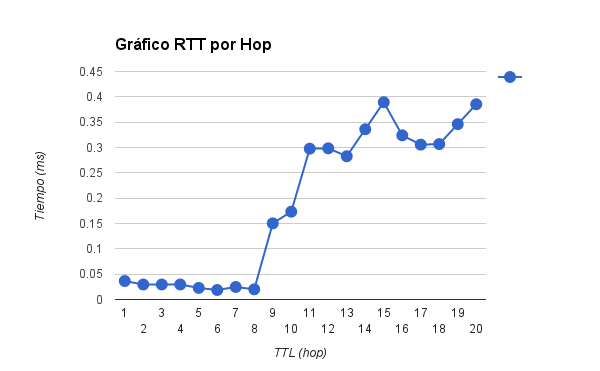
\includegraphics[width=0.7\textwidth]{img_analisis1/rtt_hop.png}
     %\label{fig:ICMPlista} 
	%\end{center} 
    
\end{figure}
\vspace{0.25cm}

%Promedio Delta RTT: 0.00588932037354, 0.223511198044, -0.0304053096771, -0.0112577915192, 0.0367794513702, 0.107529531662, -0.120579014962, 0.0107178688049, 0.107933545113, -0.0993495464325, 0.0167979955673, -0.0487000465393, 0.064146566391, 0.0933417320251, 0.0240439891815, -0.0125254392624, 0.0359566926956, -0.0348659515381, 0.0918450593948, -4.58002090454e-05, -0.00115667533875, 0.00671604824066, 0.0508928060532, -0.0580342292786, 0.00854189395905, 0.00741848945618, -0.143095983322, 0.102489104051\newline
\begin{figure}[h]
	%\begin{center}
    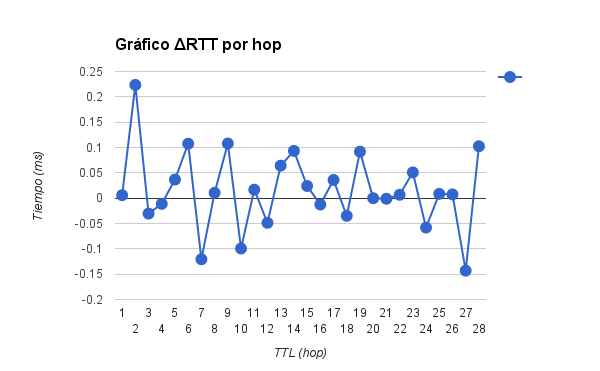
\includegraphics[width=0.7\textwidth]{img_analisis1/delta_rtt_hop.png}
     %\label{fig:ICMPlista} 
	%\end{center} 
    
\end{figure}
\vspace{0.25cm}

%Desvio Estandar Delta RTT: 0.00165442878817, 0.126023742282, 0.071172659274, 0.0745178056825, 0.1866931839, 0.180733182681, 0.0518781646894, 0.065719884364, 0.227576463877, 0.177889865429, 0.0311607993988, 0.0706603578755, 0.147728183499, 0.0762432009451, 0.0966932498659, 0.11828018604, 0.0873092181674, 0.0842616491826, 0.0484700197953, 0.112708845656, 0.0881211770851, 0.0889849976974, 0.0825379976568, 0.0601178559323, 0.0414772504639, 0.0872692906756, 0.0765956277221, 0.0546049405093\newline
\begin{figure}[h]
	%\begin{center}
    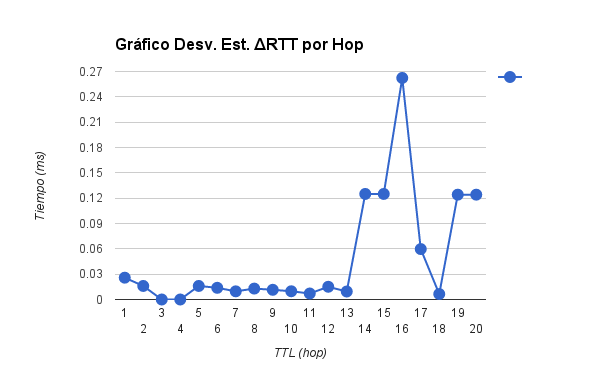
\includegraphics[width=0.7\textwidth]{img_analisis1/ds_delta_rtt_hop.png}
     %\label{fig:ICMPlista} 
	%\end{center} 
    
\end{figure}
\vspace{0.25cm}

De la muestra obtuvimos una distribuci\'on Normal, y los siguientes enlaces submarinos: nodo 2, nodo 5.\newline

Gr\'afico de mapa marcando puntos claves de la ruta:

\subsubsection{Conclusi\'on}
Explicaci\'on de los resultados obtenidos.
	\newpage

\end{document}

